\section{Discussion}
\label{ch61:discuss}

In this section I summarise and discuss the findings from the previous chapters, relating them to emerging related work and future directions.

\subsection{Making a predictable ecosystem of FAIR digital objects}
\label{ch61:ecosystem}

The main advantage of scholarly researchers publishing \emph{FAIR data} is to enable machine actionability \cite{Wilkinson 2016}, which again will accelerate further research, such as through computational workflows. 
In practice, data publishing is largely approached either by depositions in general and institutional repositories for Open Data such as Figshare and Zenodo \cite{Dillen 2019a}, or to specialised domain-specific repositories such as in biodiversity \cite{GBIF 2021}. 

European research infrastructures supporting Open Science practices are coalescing their services to form the European Open Science Cloud (EOSC) \cite{Ayris 2016}, which are embracing FAIR principles \cite{Mons 2017} and building a common framework for interoperability \cite{Kurowski 2021}. 

While existing practices for implementing FAIR have relied on the Linked Data stack, that is just one possible technology to achieve the benefits of interoperable machine actionability \cite{Mons 2017}. 

Chapter \ref{chapter:fdo} explored the emerging concept of \emph{FAIR Digital Objects} (FDO) \cite{Schultes 2019} as a potential distributed object system for FAIR data, comparing its proposed principles and current practices with the established Linked Data approach. 
As detailed in section \vref{ch3:fdo}, FDO defines a handful of constraints and guides for a predictable way to organise complex machine actionable digital entities. 

Conceptually FDO can clearly be useful for realizing FAIR principles with more active digital objects that can form a consistent ecosystem, but this opens many questions on actual FDO implementations with regards to protocols and standards.

\subsubsection{Linked Data need more constraints and consistency to be FAIR}
\label{ch61:constraints}

Examined in section \vref{ch3:ld}, the principles of \emph{Linked Data} emerged from the Semantic Web as a data-centric view with a focus on navigation and cross-site interoperability, rather than say elaborate logical inferencing systems using ontologies.  
Yet the bewildering landscape of technology choices for using RDF in data platforms means that the developers suffer and still face a steep learning curve. 
For clients consuming Linked Data from multiple sources -- \emph{Linked Data Mashup} \cite{Tran 2014} -- the situation is still baffling in that relatively small differences in identifiers, vocabularies and usage patterns across deployment result in incompatibilities that may require platform-specific workarounds and mappings \cite{Millard 2010}. 

The ecosystem of FAIR tooling is not currently mature enough to support Linked Data consumption in a user-friendly and efficient way \cite{Thompson 2020}, although recent metrics and tools for assessing \emph{FAIRness} \cite{Wilkinson 2018} can assist both data providers and consumers. 
Evaluations by EOSC has since found that FAIRness metrics can vary widely across the different assessment tools for the same data resource \cite{Wilkinson 2022a}, showing that further definitions of conventions and practices are needed for consistent Linked Data publishing and consumption. 

Making the FAIR principles achieve practical benefits for researchers and platform developers thus requires more specific constraints and broader consistency.

\subsubsection{FDOs as a distributed object system on the Web}
\label{ch61:distributed}

The framework-based comparisons in section \vref{ch3:results} considered the implementation details of both FDO and Linked Data, and evaluated to what extent either can be considered a global distributed object system. 
The findings from this research show that FDO recommendations can benefit FAIR thinking to build machine actionable ecosystems and provide stronger promises of consistency and predictability across data platforms. 

These comparisons highlighted that the Web on the other hand has a flexible, scalable and mature technology stack, which can form a solid basis for implementing FDO. 
However, if such implementation is to use Linked Data technologies, these must be constrained sufficiently in order to practically realize such an ecosystem within the FDO guidelines and without degrading the developer experience.


\subsubsection{FDOs can be implemented on the Web using Signposting}
\label{ch61:signposting}

Section \vref{ch2:meeting-fdo-principles-using-linked-data-standards} explored how the FDO principles can be achieved for Linked Data as further constraints on existing standards.
As chapter \ref{chapter:fdo} has highlighted throughout, there are many technical details remaining to be specified for FDO it to be consistently implemented according to its own principles.

If such conventions need to be evolved and specified no matter the protocol basis for FDO, this chapter argued, then it would be intuitive to build FDO on the mature Web stack, unless there was an compelling argument for alternative protocol stacks having other advantages.\footnote{
  For instance, a de-centralised, resiliant architecture and long term preservation was the motivation for the design of the Interplanetary File System (IPFS) as a \emph{Decentralized Web} \cite{Trautwein 2022}.
}

Section \ref{ch2:discussion} found that the basis of Web-based FDOs can be built using only Signposting \cite{Van de Sompel 2015,Van de Sompel 2022}, adding a couple of non-intrusive HTTP headers that are agnostic to metadata standards and serializations. An implementation of such Web-based FDOs was shown in section \ref{ch4:lightweight-fdo}. 

The Signposting approach has also been highlighted both by EOSC \cite{Wilkinson 2022a,Wilkinson 2024} and as a possible FDO configuration type \cite{Lannom 2022a}.
The FAIR-IMPACT project launched an \footurl{https://fair-impact.eu/1st-open-call-support-closed}{open call} where 14 participating institutions participated to build support for Signposting \cite{Soiland-Reyes 2023b} in their data repositories and platforms.



\subsection{RO-Crate as a developer-friendly approach}
\label{ch61:crate}

As pointed out in section \vref{ch3:ld-web}, while Linked Data is a powerful and flexible approach to publishing structured data on the Web, the developer experience of using Semantic Web technology still needs simplifications, like reducing number of choices for vocabularies and serialization formats. 

Chapter \vref{chapter:ro-crate} introduced \emph{RO-Crate} as a practical implementation of the FAIR principles for the purpose of packaging data alongside structured metadata.
The approach builds on best practices for Linked Data, however RO-Crate specifications are example-driven with simple interrelated JSON structures, and primarily use a single, general purpose vocabulary. 

This way of ``Linked Data by stealth'' means that developers don't need to be concerned about RDF implementation details, although they can at their option take advantage of RDF knowledge graph technologies like SPARQL (section \vref{ch5:linkeddata}).
Extension points are well defined, and although extending RO-Crate do require some RDF knowledge like defining namespaces, reasonable examples and vocabulary repositories are provided by RO-Crate --  developers do not for instance need to learn about ontologies nor need to deploy a web service serving multiple RDF serialisations for every described entity.



\subsubsection{Just enough Linked Data}
\label{ch61:justenough}

An important lesson from this work then is to use ``just enough'' Linked Data for the desired level of interoperability and knowledge representation.
While previous efforts to `FAIRify' largely have been concerned about representing the data values using an RDF data model, this can lead to significant effort needed in developing ontologies and vocabularies. 

RO-Crate is using \cite{schema.org} as its base vocabulary, and tries to follow its philosophy of building a lightweight semantic structure by associating many free text attributes to the same node, rather than making elaborate interconnected semantic objects.
For instance, while a \texttt{Person}'s \texttt{affiliation} ideally goes to a \texttt{Organization} with it's own URL and other attributes, in some cases, a free text string is all information available, and this can be used cirectly as the \texttt{affiliation}. 

With retrospect we can say that this reduction in semantic rigidity compared to use in OWL ontologies is a move back to the simplicity of early RDF as an open-ended model (see section \vref{ch3:semweb}), where a property can be used to point to almost anything, and RDF authors are free to use almost any term.

Another aspect that is not highlighted well in ontologies is where to stop in the formal knowledge representation of an object.
In schema.org, many properties like \url{http://schema.org/license} are defined as having the \emph{range}\footnote{Expected type of object \cite{Guha 2014}, however note that schema.org uses \url{http://schema.org/rangeIncludes} instead of \texttt{rdfs:range}, to permit multiple alternatives without the need for a union class.} of either \footurl{http://schema.org/CreativeWork}{\texttt{CreativeWork}} or \footurl{http://schema.org/URL}{\texttt{URL}}, hinting that the licence is not required to be explained as another entity with further properties, but that the attribute's primary purpose is navigation or identification. 

This would be a key aspect of Linked Data, which traditionally have had the rather undefined convention of ``follow your nose'' navigation -- a client may attempt to request any node identifier (if it is a URL), and if, with content-negotiation, it returns some RDF, then that could be integrated into a joint knowlege graph, hopefully adding more description of that node, although possibly using other vocabularies.
Signposting on the URL helps to make such navigation and expected profiles explicit.

However, ontologies used in Linked Data have not commonly indicated navigation waypoints as done in Schema.org, simply defining a property's range as a given class leaves it undefined if documents were expected to explain that node or link to its explanation. One notable exception is the Data Catalog Vocabulary (DCAT)\footnote{Although the \url{http://schema.org/Dataset} type used by RO-Crate's root entity is derived from DCAT, RO-Crate does not assume a corresponding data catalogue on the Web.} \cite{Albertoni 2020} which have navigational properties like \texttt{dcat:landingPage} (to a \texttt{foaf:Document}) and \texttt{dcat:downloadURL} (to any \texttt{rdfs:Resource}).

% Should we discuss why not DCAT?

\subsubsection{Embedding contextual information reduces need for navigation}
\label{ch61:contextual}

A divergence from common Linked Data practices is that our RO-Crate approach is making a self-described container.
Rather than assume that information will always be available from the referenced URIs, and requiring clients to crawl their way through the many identifiers to see which ones contain more information, the RO-Crate contains a minimal description of each referenced contextual entity (section \vref{ch5:contextualentities}). 

This has multiple purposes:

\begin{itemize}
    \item Simplify user interfaces, e.g. show a human-readable label and type before the user chooses to click the link.
    \item Vocabulary adaptation, for instance describing with schema.org in the crate, what was expressed in FOAF vocabulary at the URI.
    \item Unify descriptions of semantic artefacts and web pages. 
          Making ``ad-hoc'' semantic artefacts within the crate where none exited beforehand.
    \item Embed ``as of at time of writing'' descriptions for longevity. 
          An RO-Crate is self-contained and can be archived independently, and embedding contextual information reduces cross-organizational service dependencies (at the risk of outdated information).
\end{itemize}

Several of these reasons are also organizational in nature, reflecting back on the EOSC Interoperability Framework (section \vref{ch3:eosc-interoperability-framework}) -- rather than requiring for instance the Research Organization Registry \footurl{https://ror.org/}{(ROR)} to add Linked Data representations of organizations, one can be made ad-hoc by the RO-Crate's author, and contained by the crate as a contextual entity. 

This ability to describe a referenced entity locally is also a workaround for the chicken-and-egg problem of creating and linking Linked Data resources that vocabulary-wise are cross-related both ways. For instance orcid.org recently added schema.org content negotiation, but \emph{after} RO-Crate started describing people using the \url{http://schema.org/Person} type and ORCID identifiers.\footnote{
  One of my earlier code contributions to ORCID already established content-negotiation to RDF -- but using the classical FOAF vocabulary \cite{Brickley 2014}.
  Slightly inconsistent with Semantic Web principles\footnotemark, the registry is currently returning \emph{Person} descriptions in different semantic models depending on the requested serialization. \\
  \url{https://github.com/ORCID/ORCID-Source/blob/main/CONTENT_NEGOTIATION.md}} 

% Yes finally I needed a footnote in a footnote!  
\footnotetext{Signposting \cite{Van de Sompel 2022} would indicate alternative vocabularies using distinct \texttt{profile} URIs.} 

\subsubsection{FDO ecosystems need to permit flexible references}
\label{ch61:references}

When reflecting on the above contextualization from the propositions of FAIR Digital Objects as covered back in chapter \ref{chapter:fdo}, we can predict a problem if every reference from an FDO must go to another pre-existing FDO (or at least a registered PID), in that there must then be a linear order of FDO creation within an ecosystem of compatible FDO types.
A strict reading of the FDO principles means implementations cannot utilise the established human-readable Web for bootstrapping.
This risks large cross-organizational delays with a stronger need for collaboration and coordination, or alternatively, starting with a smaller FDO data models that can gradually evolve to add more navigation, when and if registries appear with FDO interfaces. 

The emphasis on strong typing in FDOs also means that seemingly incompatible types (for instance developed by the biodiversity community vs. those from genomics communities) lead to a split of the PID space of referenceable objects from a given type of FDOs.  Counter to this, the current FDO recommendations for attributes and types \cite{Blanchi 2023} do not require specification of the \emph{range} of an attribute to be a PID of an FDO, and as current FDO type declarations have been relatively lightweight (textual descriptions only), they are flexible enough to permit URLs to any Web resource or existing Linked Data concepts.  

There is a concern, however, that some FDO serializations using the Handle system and key-value attributes cannot distinguish between string literals and object references.
Combined with the use of PID references expressed as handles rather than as a URIs (e.g. \texttt{21.14100/2fcf49d3-0608-3373-a47f-0e721b7eaa87} instead of \url{https://hdl.handle.net/21.14100/2fcf49d3-0608-3373-a47f-0e721b7eaa87}), this means that machine actionability suffers, in that the string value is not typed to what kind of reference it may or may not be, or in what PID system. Compare this with listing \vref{ch3:triples} where the RDF syntax distinguishes literal strings from object references -- in Handle-based FDOs, machine-actionable navigation is only possible by understanding the attributes of the FDO type, yet as highlighted in the previous paragraph these type definitions are not directly machine-actionable themselves.

In schema.org we find a similar challenge with properties permitting both string values and object references. \url{http://schema.org/keywords} is perhaps the most ambiguous, as it permits \texttt{Text}\footnote{To conflate matters, the \texttt{keywords} property can be repeated, but also allows multiple keywords within a single comma-separated string.}, but also \texttt{URL} or \texttt{DefinedTerm}.
The two latter cases are both intended for referencing controlled vocabularies, with the distinction that a \texttt{DefinedTerm} is defined explicitly within the referenced object, while the defined term is implied if only the URL is provided.
JSON-LD contexts have the possibility of enforcing object references (\texttt{"@type: "@id"}), but this cannot be used in this case as freetext strings are also permitted.
The result is that a freetext keyword that just looks like a URL cannot be distinguished from an intended URL reference, similar to the FDO Handle example in the previous paragraph.

In order to reduce such ambiguity and multiple developer choices, in RO-Crate all object references are in JSON-LD object form (as we saw in Listing \vref{ch5:lis1}), and the RO-Crate context do not have any \texttt{@type} shortcuts for implicit references.
RO-Crate 1.2 will also recommend that \footurl{https://www.researchobject.org/ro-crate/1.2-DRAFT/metadata.html\#common-principles-for-ro-crate-entities}{all entities} have a type, identifier and human-readable name. 


\subsubsection{Profiles restrict general flexibility to gain specific predictability}
\label{ch61:profiles}

Section \vref{ch5:inuse} showed how RO-Crate is adopted by different scientific domains. 
Since the publication of the corresponding manuscripts in chapter \ref{chapter:ro-crate}, RO-Crate has also been used by the \footurl{https://www.researchobject.org/ro-crate/in-use/LDaCA.html}{Language Data Commons of Australia} \cite{Smith 2022} building language corpa, \footurl{https://www.researchobject.org/ro-crate/in-use/survey-ontology.html}{Survey Ontology} \cite{Scrocca 2021} describing surveys, \footurl{https://nfdi4plants.org/content/learn-more/annotated-research-context.html}{DataPlant} for plant experiments, \footurl{https://w3id.org/cpm/ro-crate}{distributed provenance} of biological specimens \cite{Wittner 2020,Wittner 2023a,Wittner 2023b}, \footurl{https://w3id.org/ro/doi/10.5281/zenodo.6913045}{COVID-19 causal inferences} to compare public health interventions internationally \cite{Meurisse 2023}, and \footurl{https://w3id.org/5s-crate/0.4}{Trusted Research Environments} for controlled workflow computation on sensitive health data. Several of these use cases have also expanded RO-Crate with additional terms from schema.org or defined in corresponding RO-Crate profiles. The span of these domains shows that RO-Crate is flexible for a range of use cases and can be adopted by developers not familiar with Semantic Web technologies.

The discussion of strictness vs flexibility in section \vref{ch5:strictness-vs-flexibility} highlighted the tension between a flexible open-ended model and the predictability needed to consistently create and consume content expressed by the model.
While RO-Crate itself can be seen as a restriction of the more open-ended JSON-LD and schema.org, its extensibility points still allow different use cases to expand on those conventions.  

Section \vref{ch5:profiles} detailed how semi-formalised profiles can be gradually formed to at first \emph{duck-type} a class of RO-Crates that have similar properties.
Later work has formalised this as \footurl{https://www.researchobject.org/ro-crate/1.2-DRAFT/profiles}{Profile Crate} to capture the profile itself as a separate crate. This have now evolved to use the W3C Profiles Vocabulary \cite{Atkinson 2019} to explicitly link to vocabularies, mappings and importantly constraints expressed as RDF Shapes \cite{Soiland-Reyes 2023d}. 
This turns RO-Crate profiles into machine-actionable type definitions, from which existing RDF tooling can do for instance validation. 
Figure \ref{ch61:fig:profilecrate} shows how the usage of \emph{roles} within the profile crate indicates the purpose of the constituent parts.
Roles are here particularly important as many of these Semantic Web resources are expressed in the same file format (e.g. \texttt{text/turtle}) and may be used for different purposes (e.g.
SKOS is used to represent either a \emph{mapping} or a \emph{vocabulary} \cite{Isaac 2009}).

\begin{figure}[htb]
    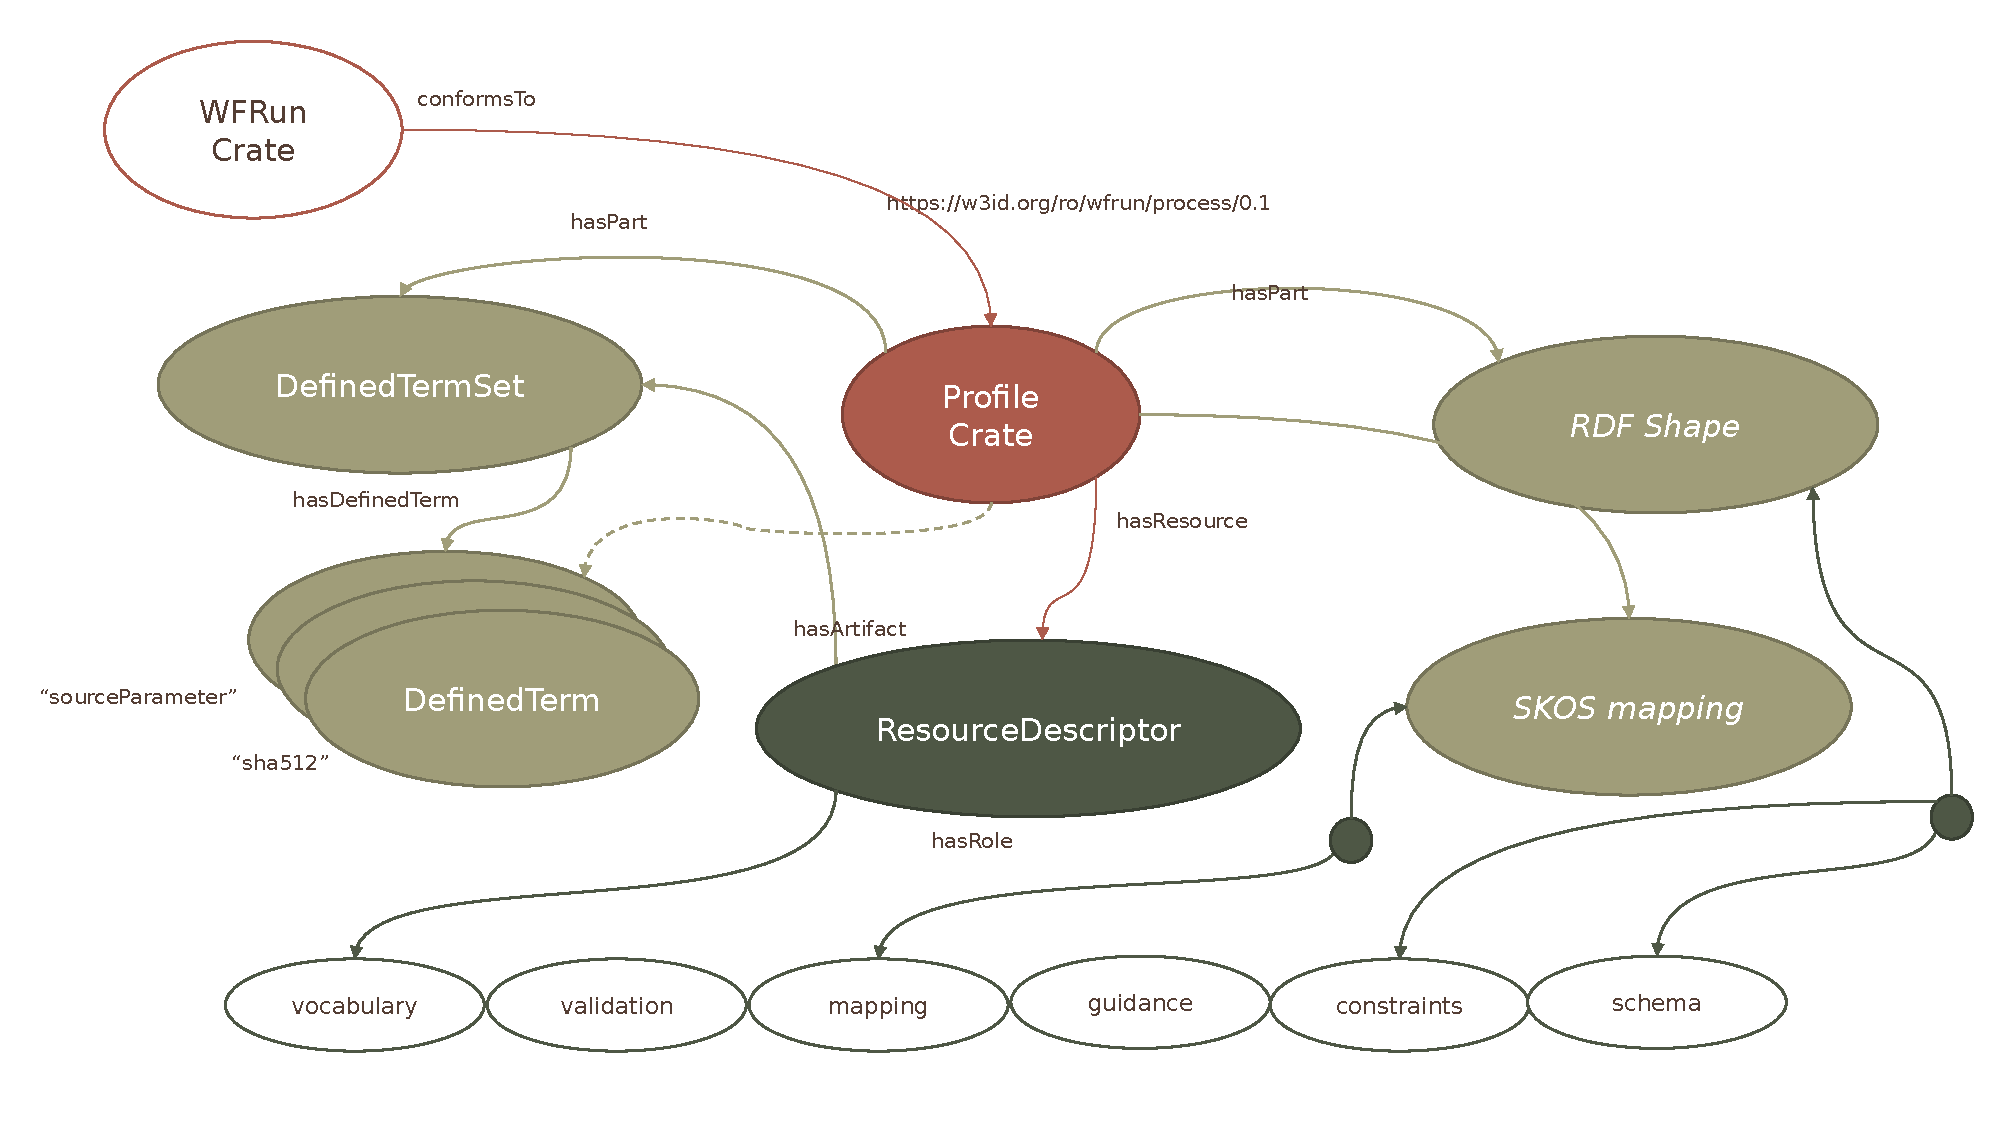
\includegraphics[width=\textwidth]{figures/ch09/profile-crate.pdf}
      \caption[Example of Profile Crate]{\textbf{Example of Profile Crate for Workflow Run Crate}. 
      An RO-Crate \emph{WFRun Crate} declares conformance with a given RO-Crate profile. 
      Resolving the profile URI retrieves the \emph{Profile Crate}, which parts include an \emph{RDF Shape}, an \emph{SKOS mapping} and a \emph{DefinedTermSet}. 
      By using the indirection of \emph{ResourceDescriptor} from the Profiles Vocabulary \cite{Atkinson 2019}, the roles of each of these artefacts are defined, e.g. \emph{constraints}. 
      The embedded \emph{vocabulary} as a \emph{DefinedTermSet} defines ad-hoc terms like \emph{sourceParameter} used by the Workflow Run Crate\footnotemark~ profile \cite{Leo 2023b}.
      }
    \label{ch61:fig:profilecrate}
  \end{figure}
\footnotetext{\url{https://w3id.org/ro/wfrun/process/0.2}}

While profiles are at first lightweight indicators of common conventions for a class of crates (which may be implicit or explicit), they can be gradually formalised in a \emph{eat own dogfood} way through another RO-Crate, optionally taking advantage of existing Semantic Web technology that enable for instance strict validation of domain-specific RO-Crates.


\subsubsection{One vocabulary is not enough, but one profile may suffice}
\label{ch61:oneprofile}

RO-Crate relies heavily on \cite{schema.org} as its main vocabulary, but as highlighted in section \vref{ch5:futurework} and \vref{ch61:profiles}, domain-specific usage will eventually need to define their own terms in order to be specific enough for their use cases. However, we have found it is important to ensure a developer-friendly approach when specifying such profiles for RO-Crate -- earlier work on \footurl{https://www.researchobject.org/ro-crate/1.1/appendix/jsonld.html\#adding-new-or-ad-hoc-vocabulary-terms}{ad-hoc terms} in RO-Crate used a simple CSV approach to be added to the \footurl{https://github.com/ResearchObject/ro-terms}{ro-terms} namespace.  

As with other aspects of RO-Crate, there is a gradual approach towards Linked Data practices. While conventional wisdom in Semantic Web would be to sit down and make your own ontology following design patterns \cite{Blomquist 2009,Poveda 2010} and best practices for deployment \cite{Matentzoglu 2022}, in RO-Crate philosophy that would be more of a last resort. The middle of the ground is therefore adding the ad-hoc vocabulary directly to the profile crate, as shown in figure \vref{ch61:fig:profilecrate}. In this approach a single profile URI can, through Linked Data and Signposting, play the role of:

\begin{itemize}
  \item Human-readable documentation of conventions (negotiated to HTML preview).
  \item List of software and repositories the profile is intended for.
  \item List of additional schema.org types and properties utillised by the profile.
  \item Indication of which content is expected in the crate (e.g. a Workflow).
  \item Validation of a manifest conforming to the profile.
  \item Vocabulary definitions of additional terms.
  \item JSON-LD context which namespaces the additional terms  (as any JSON-LD document can also be a JSON-LD context \cite{Sporny 2020}).
\end{itemize}

It should be reasonable to expect developers able to make RO-Crates with their own additional terms to also be able to make a lightweight Profile Crate once those terms have stabilised. Developers with deeper familiarity with Semantic Web technologies can expand the profile capabilities to use existing ontology methodologies, in which case it would be preferrable to aggregate separate semantic artefacts from the Profile Crate rather than embedding them in the RO-Crate Metadata File.

In the FAIR-IMPACT project we are evaluating if the Profile Crate approach is also suitable for FAIR publishing of semantic artefacts themselves, e.g. ontologies and mappings. This is an attractive proposal because such artefacts are also becoming multifaceted, with multiple formats and profiles (e.g. an ontology expressed with OWL2 RL in RDF Turtle syntax), documentation and similar attribution and provenance challenges which RO-Crate is built to handle.

\subsection{Future RO-Crate directions}
\label{ch61:rocratefuture}
In this section we consider future directions for RO-Crate and ongoing RO-Crate adaptations not covered by section \ref{ch5:packaging-research-artefacts-with-ro-crate}.


\subsubsection{User applications are needed for researchers to generate FAIR Research Objects}
\label{ch61:applications}

RO-Crate and its best practices can be considered a type of \emph{middleware} used by application developers to capture and transmit metadata and relate data files that together form some tangible unit (a \emph{Research Object} \cite{Bechhofer 2013}). While RO-Crate have already been implemented by several repositories and applications such as workflow systems, it is important to also consider the role of user applications in order to increase adoptation of FAIR research objects by scholars in general.

\paragraph{Template-based crates with ya2ro}
Futher work by the RO-Crate community has created more user-fronting tools such as \footurl{https://github.com/oeg-upm/ya2ro}{Pavel 2023,} which given metadata and identifier in a YAML\footnote{
  YAML is a file format with the same data model as JSON, but with a more readable syntax, e.g. using indentation instead of quoted strings.  \url{https://yaml.org/}} 
file can retrieve contextual metadata from ORCID, GitHub and DOI registries and build and publish a completed RO-Crate \cite{Pavel 2023}.   
While this technology still requires some understanding of editing, it is intended to be more approachable to data scientists and for use with simple Web publishing platforms like \footurl{https://pages.github.com/}{GitHub Pages.} The GitHub Action \footurl{https://github.com/marketplace/actions/ro-crate-preview}{ro-crate-preview} also automate HTML preview generation of crates on GitHub Pages.

\paragraph{Editing and publishing RO-Crate in ROHub}
The repository \footurl{https://www.rohub.org/}{ROHub} \cite{Garcia-Silva 2019} has recently added RO-Crate import and export \cite{Fouilloux 2023}, and provides both a browseable repository for publishing crates, but also interactive and collaborative editing of its metadata. 
In this use case, RO-Crate plays the role as an exchange and archiving format, as the hub stores the crates in general-purpose repositories Zenodo and B2Share which do not have the facility to keep the granular metadata expressed within the RO-Crate metadata file. As detailed in \cite{Fouilloux 2023}, a series of templates assist users in creating research objects with particular content and annotations. 

\paragraph{Making ad-hoc vocabularies in Crate-O}\label{ch61:crate-o}
The \footurl{https://language-research-technology.github.io/crate-o/}{Crate-O} tool has been developed by Language Data Commons of Australia \footurl{https://ldaca.edu.au/}{(LDaCA)} as a general-purpose RO-Crate editor and successor to Describo \cite{La Rosa 2021d} and Describo Online \cite{La Rosa 2021c}. 
This tool can describe any folder and resources from the Web as an RO-Crate, supporting any schema.org type and property, pluggable with any rdfs vocabularies \cite{Guha 2014}. 
Notably this tool is also intended for creation of such vocabularies, and is thus a lightweight user interface for building a Profile Crate (section \vref{ch61:profiles}) using Schema.org style Schemas\footnote{
  It is notable that schema.org's own vocabulary definition use rdfs directly for Linked Data interoperability, 
  rather than its own \url{http://schema.org/Class}, \url{http://schema.org/Property}, or the SKOS-like \url{http://schema.org/DefinedTerm}. 
  On property definitions, SoSS use \url{http://schema.org/domainIncludes} and \url{http://schema.org/rangeIncludes} to avoid union classes for alternative domain/range types, which can clutter OWL/RDFS equivalent properties.} 
\footurl{https://schema.org/docs/schemas.html}{(SoSS)}.

\paragraph{Executable papers can fully represent their computation using RO-Crate}
\label{ch61:livepublication}

\footurl{https://livepublication.github.io/LP_Pub_LID/}{LivePublication} \cite{Ellerm 2023} is a proof of concept of an \emph{executable paper}, which interactive visualization and statistical calculations can be regenerated on the fly taking into consideration data sources updated after the paper's publication date. A \footurl{https://livepublication.github.io/LP_Pub_OrchestrationCrate/}{corresponding RO-Crate} is the mechanism to enable this execution on the Globus infrastructure through an innovative use of individual RO-Crates and containers for each computable element of the paper, nested within a top-level Crate for the paper.

This novel approach shows how it is possible to use RO-Crate as an machine-actionable object, which do not rely on bundling an underlying workflow representation in an existing workflow language.  

\subsubsection{Web-based FDOs can use RO-Crate for its metadata}
\label{ch61:webfdo}

Section \vref{ch4:lightweight-fdo} argues that many of the FDO requirements \cite{Anders 2023} for metadata can be implemented as \emph{RO-Crate FDOs} (section \vref{ch8:fair-packaging-of-researchworkflow-objects-with-ro-crate}), with FAIR Signposting \cite{Van de Sompel 2015,Van de Sompel 2022} assisting navigation from persistent identifiers, and the RO-Crate containing the metadata. 

This approach was first implemented in the repository WorkflowHub \cite{Goble 2021,Wittenburg 2022}, and in the FDO Forum \cite{Van de Sompel 2023} suggests RO-Crate with Signposting as a modern update to his OAI-ORE\footnote{OAI-ORE was also used by earlier Research Object approaches \cite{Belhajjame 2015,Soiland-Reyes 2014} to capture the aggregation aspect of ROs.} approach from 2008 \cite{Lagoze 2008}.  
RO-Crate FDOs are being further developed within the Horizon Europe projects \footurl{https://eurosciencegateway.eu/}{EuroScienceGateway} \cite{Soiland-Reyes 2022f} and \footurl{https://fair-impact.eu/}{FAIR-IMPACT} \cite{Goble 2022}.

RO-Crate FDOs complements the findings of section \vref{ch61:signposting}, in that RO-Crate provides FDO with a generic metadata framework and a serialization that can work both for FDOs on the Web and with legacy Handle/DOIP approaches --  this metadata role for RO-Crate in the FDO ecosystem is also highlighted by \cite{Wittenburg 2023b}.

Some extra considerations is rightly needed on identifiers to reduce relative paths challenges with  RO-Crate FDOs -- for this purpose, the next specification \cite{RO-Crate 1.2} introduce a distinction between an \footurl{https://www.researchobject.org/ro-crate/1.2-DRAFT/structure.html\#attached-ro-crate}{attached RO-Crate} (\emph{has some root directory containing other files referenced by relative paths, possibly archived in a ZIP or exposed on the Web}) and a \footurl{https://www.researchobject.org/ro-crate/1.2-DRAFT/structure.html\#detached-ro-crate}{detached RO-Crate} (\emph{no defined root directory, all references are absolute}). 
This \emph{detached} style is suitable for an FDO architecture, even for use within APIs which do not lend themselves to relative path references (such as DOIP-over-HTTP \cite{CNRI 2023a}).
RO-Crate 1.2 also define methods for \footurl{https://www.researchobject.org/ro-crate/1.2-DRAFT/appendix/relative-uris.html}{converting between attached/detached} crates using standard JSON-LD tooling, showing another advantage of using Linked Data as basis for RO-Crate. 


\subsubsection{How FAIR are RO-Crates?}
\label{ch61:fair-crates}

FAIROs \cite{González 2022} is a framework for calculating a ``FAIRness'' score for research objects. For RO-Crate evaluation this puts additional requirements on the use of persistent identifier for the RO-Crate, and that the core metadata of the crate (e.g. licensing) is provided. These aspects are important for ensuring FDO machine actionability of RO-Crates.

Another aspect of FAIRness for RO-Crate is if extensions are themselves following FAIR principles (RDA-I2-01M \emph{Metadata uses FAIR-compliant vocabularies}).  The Profile Crate specifications for \footurl{https://www.researchobject.org/ro-crate/1.2-DRAFT/profiles\#extension-vocabularies}{extension vocabularies} recommends the use of \texttt{DefinedTerm} or \texttt{DefinedTermSet} as a mechanism to ``import'' an existing term or vocabulary to the profile, allowing a neutral way to define these terms independent of their ontology technology. There is some tension with Crate-O's   ``Schema.org style Schemas'' (see section \vref{ch61:crate-o}) which desired compatibility with \texttt{rdfs:Class} and \texttt{rdfs:Property} and wide-spread RDFS tooling -- the RO-Crate community consensus is to use the rdfs types when the term is \emph{defined} by the profile rather than imported and to avoid the RDFS-like \url{http://schema.org/Class} and \url{http://schema.org/Property} overall.

The use of profiles, and particularly nested profiles as in figure \vref{ch54:fig:profile_venn}, makes validation of RO-Crates more complex. An initial approach of \footurl{https://github.com/ResearchObject/runcrate/pull/17}{ShEx validation in runcrate} extended the \footurl{https://github.com/ResearchObject/ro-crate-validator-py}{ro-crate-validator-py} library to use ShEx based validation \cite{Baker 2019} depending on declared WRROC profiles.
\footurl{https://s11.no/2023/comp66090/profiles/}{Future work} is planned to further investigate this using a combination of Semantic Web and RDF Shapes technologies, possibly using hierarchical profile validation with \footurl{https://github.com/surroundaustralia/cheka}{Cheka} but based on the crate's declared \texttt{conformsTo} statements.


\subsubsection{RO-Crate can build collections of digital objects}
\label{ch61:collections}

RO-Crate has also been proposed as a generic mechanism for FDO Collections \cite{Soiland-Reyes 2023d}, as an aggregator of FDOs by their PIDs. Such collections add a similar challenge in FDO as in Linked Data, in that clients may need to resolve an excessive number of persistent identifiers (see section \vref{ch20:avoid-lots-of-requests}) to FDOs which may be of different semantic types. 
Using a detached RO-Crate for such collections, the bibliographic metadata of each PID can be directly embedded and normalised to a single vocabulary, reducing client needs for recursive queries and type mappings. 
 
Work on building large data citations as a ``reliquary'' -- a \emph{container of persistent identifiers (PIDs)} \cite{Buck 2022} -- started from the earth science domain with AGU's \footurl{https://data.agu.org/DataCitationCoP/}{Data Citation Community of Practice} and continues in RDA's \footurl{https://www.rd-alliance.org/groups/complex-citations-working-group}{Complex Citation Working Group}. In this approach RO-Crate is being considered as a promising implementation to capture large number of citations along with minimal metadata, including licensing and attribution. Here a main motivation is to avoid excessive lists of data citations for scholarly publications following processing of aggregated datasets from repositories such as GBIF \cite{GBIF 2021}, while still propagating each dataset's FAIR metadata (as required by the Creative Commons Attribution licence) through the indirection of a collection. There is a potential overlap with workflow run provenance, although a workflow is not required by reliquaries.


\subsubsection{Mutable FDOs can be captured in knowledge graphs using RO-Crate}
\label{ch61:datalakes}

Knowledge Enhanced Digital Objects \footurl{https://github.com/luoyu357/KEDODataLake}{(KEOD)} \cite{Luo 2022} is an experimental approach of building a data lake using a combination of knowledge graphs, RO-Crate and PID records \cite{Luo 2023}. This is effectively an FDO implementation: A KEDO PID is a Handle that identifies a KEDO Object, described using a KEDO RO-Crate. This crate again has \emph{internal RO-Crate}s as parts, which records a combination of \emph{Features} and \emph{Insights}. The distinction is that features are mainly fixed at digital object creation and considered directly describing the object's nature, while insights can be discovered later from further processing and linkage. This approach solves a mutability problem in FDOs, as the KEOD system only allows insights to be added along with provenance that connect PIDs when KEDOs evolve. Files in a KEDO RO-Crate are stored locally, and each recorded with a Handle PID within the crate.

This KEOD setup of multiple graphs forming a single knowledge unit can be considered analoguous to nanopublications \cite{Kuhn 2021} but for FDOs. Indeed using nanopublication to capture FDOs of digital twins has also been proposed \cite{Schultes 2022}, however, that use a different distributed architecture where the PIDs for nanopublications are generated by cryptographically hashing their content \cite{Kuhn 2021}.


\subsubsection{Distributed architectures for FAIR Digital Objects can use detached crates}
\label{ch61:dpid}

The \footurl{https://docs.desci.com/}{DeSci Nodes} system has been developed by the \footurl{https://www.descifoundation.org/}{DeSci foundation}, where \footurl{https://www.dpid.org/}{dPID} (distibuted Persistent Identifier) act  as an overlay of the Interplanetary File System (IPFS) \cite{Trautwein 2022}. 
Users can interact with the DeSci platform for building and publishing Research Objects, and the \footurl{https://docs.desci.com/learn/open-state-repository/metadata}{DeSci metadata} are exposed as a \footurl{https://www.researchobject.org/ro-crate/1.2-DRAFT/structure.html\#detached-ro-crate}{detached RO-Crate} with IPFS references (see \footurl{https://beta.dpid.org/46?jsonld}{example dPID}). 
DeSci Nodes have documented a \footurl{https://docs.desci.com/learn/fair-data/fair-compliance/desci-nodes-fip}{FAIR Implementation Profile} (FIP) \cite{Schultes 2020} documenting compliance with FAIR principles. 

This is a novel FAIR Digital Object implementation that challenges both the traditional centralised FDO approach using the Handle system, as well as the mostly Web-based RO-Crate ecosystem covered in section \vref{ch5:packaging-research-artefacts-with-ro-crate}. It remains to be independently verified if the decentralisation of IPFS is effectively constrained by access through a centralised API, or if dPIDs can be retrieved from multiple independent resolvers.

The use of detached crates has also been utilised by the \footurl{https://www.researchobject.org/ro-crate/in-use/LDaCA.html}{Language Data Commons of Australia Program}, where RO-Crate is part of navigating centralised API resources, rather than a standalone publication on the Web. In both of these approaches, additional FDO measures such as using persistent identifiers and validation against profiles become important. 


\subsection{Workflows capture computational methods}
\label{ch61:workflow}

Chapter \vref{chapter:workflows} explored in depth different ways in which FAIR Digital Objects and RO-Crate are applied to computational workflows, in effect capturing the computational methods in a FAIR Research Object. 


\subsubsection{Workflows can be constructed of FAIR digital objects}
\label{ch61:workflowfdo}

As introduced in section \vref{intro:rq3}, we have previously proposed the concept of \emph{FAIR Computational Workflows} \cite{Goble 2020}. 
That work expands on the well-established motivations for using scientific workflow systems \cite{Möller 2017,Atkinson 2017}, such as supporting Automation, Scalable execution, Abstraction, and Provenance \cite{Ludäscher 2016}, and highlights that workflows themselves benefit from and contribute to FAIR data, for instance providing metadata for describing workflow outputs. 
In addition workflow themselves can be considered digital objects that should be shared as a reproducible computational method.

Applying the FAIR principles for workflows in practice has however revealed additional challenges, such as lack of clarify of what constitutes a \emph{workflow} as opposed to FAIR Research Software in general \cite{Katz 2021b}, or reduced reusability when the workflow requires unwritten, human-centric operations between computational steps (e.g. trivial file column manipulations) \cite{Wilkinson 2022b}. 

In developing the repository \footurl{https://workflowhub.eu/}{WorkflowHub} \cite{Goble 2021} we emphasised the importance of preserving and publishing not just executable workflow definitions, 
but their structured descriptions independent of workflow formats as well as further references to external sources, software required (including the workflow engine).
For this we developed the Workflow RO-Crate Profile \cite{Bacall 2022}, which became a foundational format for more specific workflow execution profiles (section \vref{ch54:wrroc}).

One aspect that makes workflow management systems different from research software in general, is that the they frequently encourage modularization, in that the composition of steps also can reflect the analytical process that is intended by the scientists.
Mature workflow systems like Galaxy \cite{Galaxy 2022} provide a large collection of re-usable components that wrap underlying command line tools and make them interoperable without manual adjustments. 
In CWL  \cite{Crusoe 2022}, tool definitions include not just execution details, but also structured input/output definitions, allowing them to be reused and combined in multiple workflows.

Section \vref{ch6:making-canonical-workflow-building-blocks-interoperable-across-workflow-languages} explored how such building blocks can themselves be considered FAIR digital objects. These assist workflow systems in propagating rich metadata about tools and their analytical purpose, but also allows building blocks to be reused across workflow systems. This in effect means that a \emph{canonical workflow} \emph{Wittenburg 2021} can be implemented in different workflow languages, each executing the same \emph{canonical steps} in the same way. Given that FAIR Digital Objects emphasize machine-actionability, and we can consider workflows as FDOs, it is important to have the ability not just to reliably re-execute a workflow, but even re-use its constituent steps. 


\subsubsection{Building FDOs incrementally challenges typing constraints}
\label{ch61:buildingfdo}

Sections \vref{ch8:the-specimen-data-refinery} and \vref{ch7:incrementally-building-fair-digital-objects-with-specimen-data-refinery-workflows} showed another aspect of using such building blocks, where FDOs are the unit of communication between steps in the workflow. 
This approach is pushing the envelope of FAIR Digital Objects concept, by having the FDO built incrementally by different stages of the specimen digitization pipeline, and exchanged only within the workflow system before it is ready to be published. 
This scenario, where we experimented with strict validation with JSON Schema for every step, highlighted limitations of having larger composite FDO object types, as intermediate FDOs would not validate without significantly softening the schema.
In effect the Specimen Data Refinery (SDR) workflow can be considered as a variant of the classic \emph{Builder pattern} \cite[pp. 97--106]{Gamma 1995}, which gradually constructs an object through a series of operations on an intermediate object (the builder).
However, as highlighted by section \vref{ch7:fdo-lessons}, ducktyping-like profiles/interfaces are needed for typing incremental FDOs, to ensure that a later workflow step receives a partial FDO with the expected fragments populated, otherwise workflow users would be able to compose steps with the FDO in an invalid state. 

The later section \vref{ch54:the-workflow-run-ro-crate-profiles} showed how RO-Crate profiles for workflow provenance FDOs can be staggered for different granularity levels, but that is more akin to a class hierarchy, as each level builds on previous complete levels.  The Five Safes Crate profile (section \vref{ch54:trusted-workflow-run-crate}) however, has a similar incremental pattern as the SDR FDOs, and the different review states should be performed in a particular order. Enforcing this for typing purposes may require explicit rule-based abstract state machines (ASM) \cite{Gurevich 1995}, as has been demonstrated for Linked Data with ASM4LD \cite{Käfer 2018a,Käfer 2018b}.


\subsubsection{Flexible profiles increase adaptability of interoperable provenance}
\label{ch61:provenance}


Section \vref{ch54:wrroc} introduced the Workflow Run Crate (WRROC) profiles for capturing workflow provenance. It was highlighted that the multiple levels were designed to ease adoptability -- indeed the different WRROC implementations (section \vref{ch54:implementations}) have chosen  profiles depending on the provenance available to that particular engine. 
In addition, some implementations had to utilise optionality of some attributes, for instance to handle dynamic workflows. 

In addition the \emph{Process Run Crate} profile was shown to be suitable also for ``manual workflows'' where processes are executed by hand, as illustrated by figure \vref{ch61:fig:baseline-usecase}.
In this example, the process run is only a small part of the crate, namely to generate the synthetic dataset, but of bigger importance in this crate is the causal model that explains to humans the relationships that led to the synthetic dataset. 
There is no overall computational workflow as the individual computational steps are performed with human interaction; however, this also means the RO-Crate metadata must be created by human interaction.



\begin{landscape}
\begin{figure}[p]
  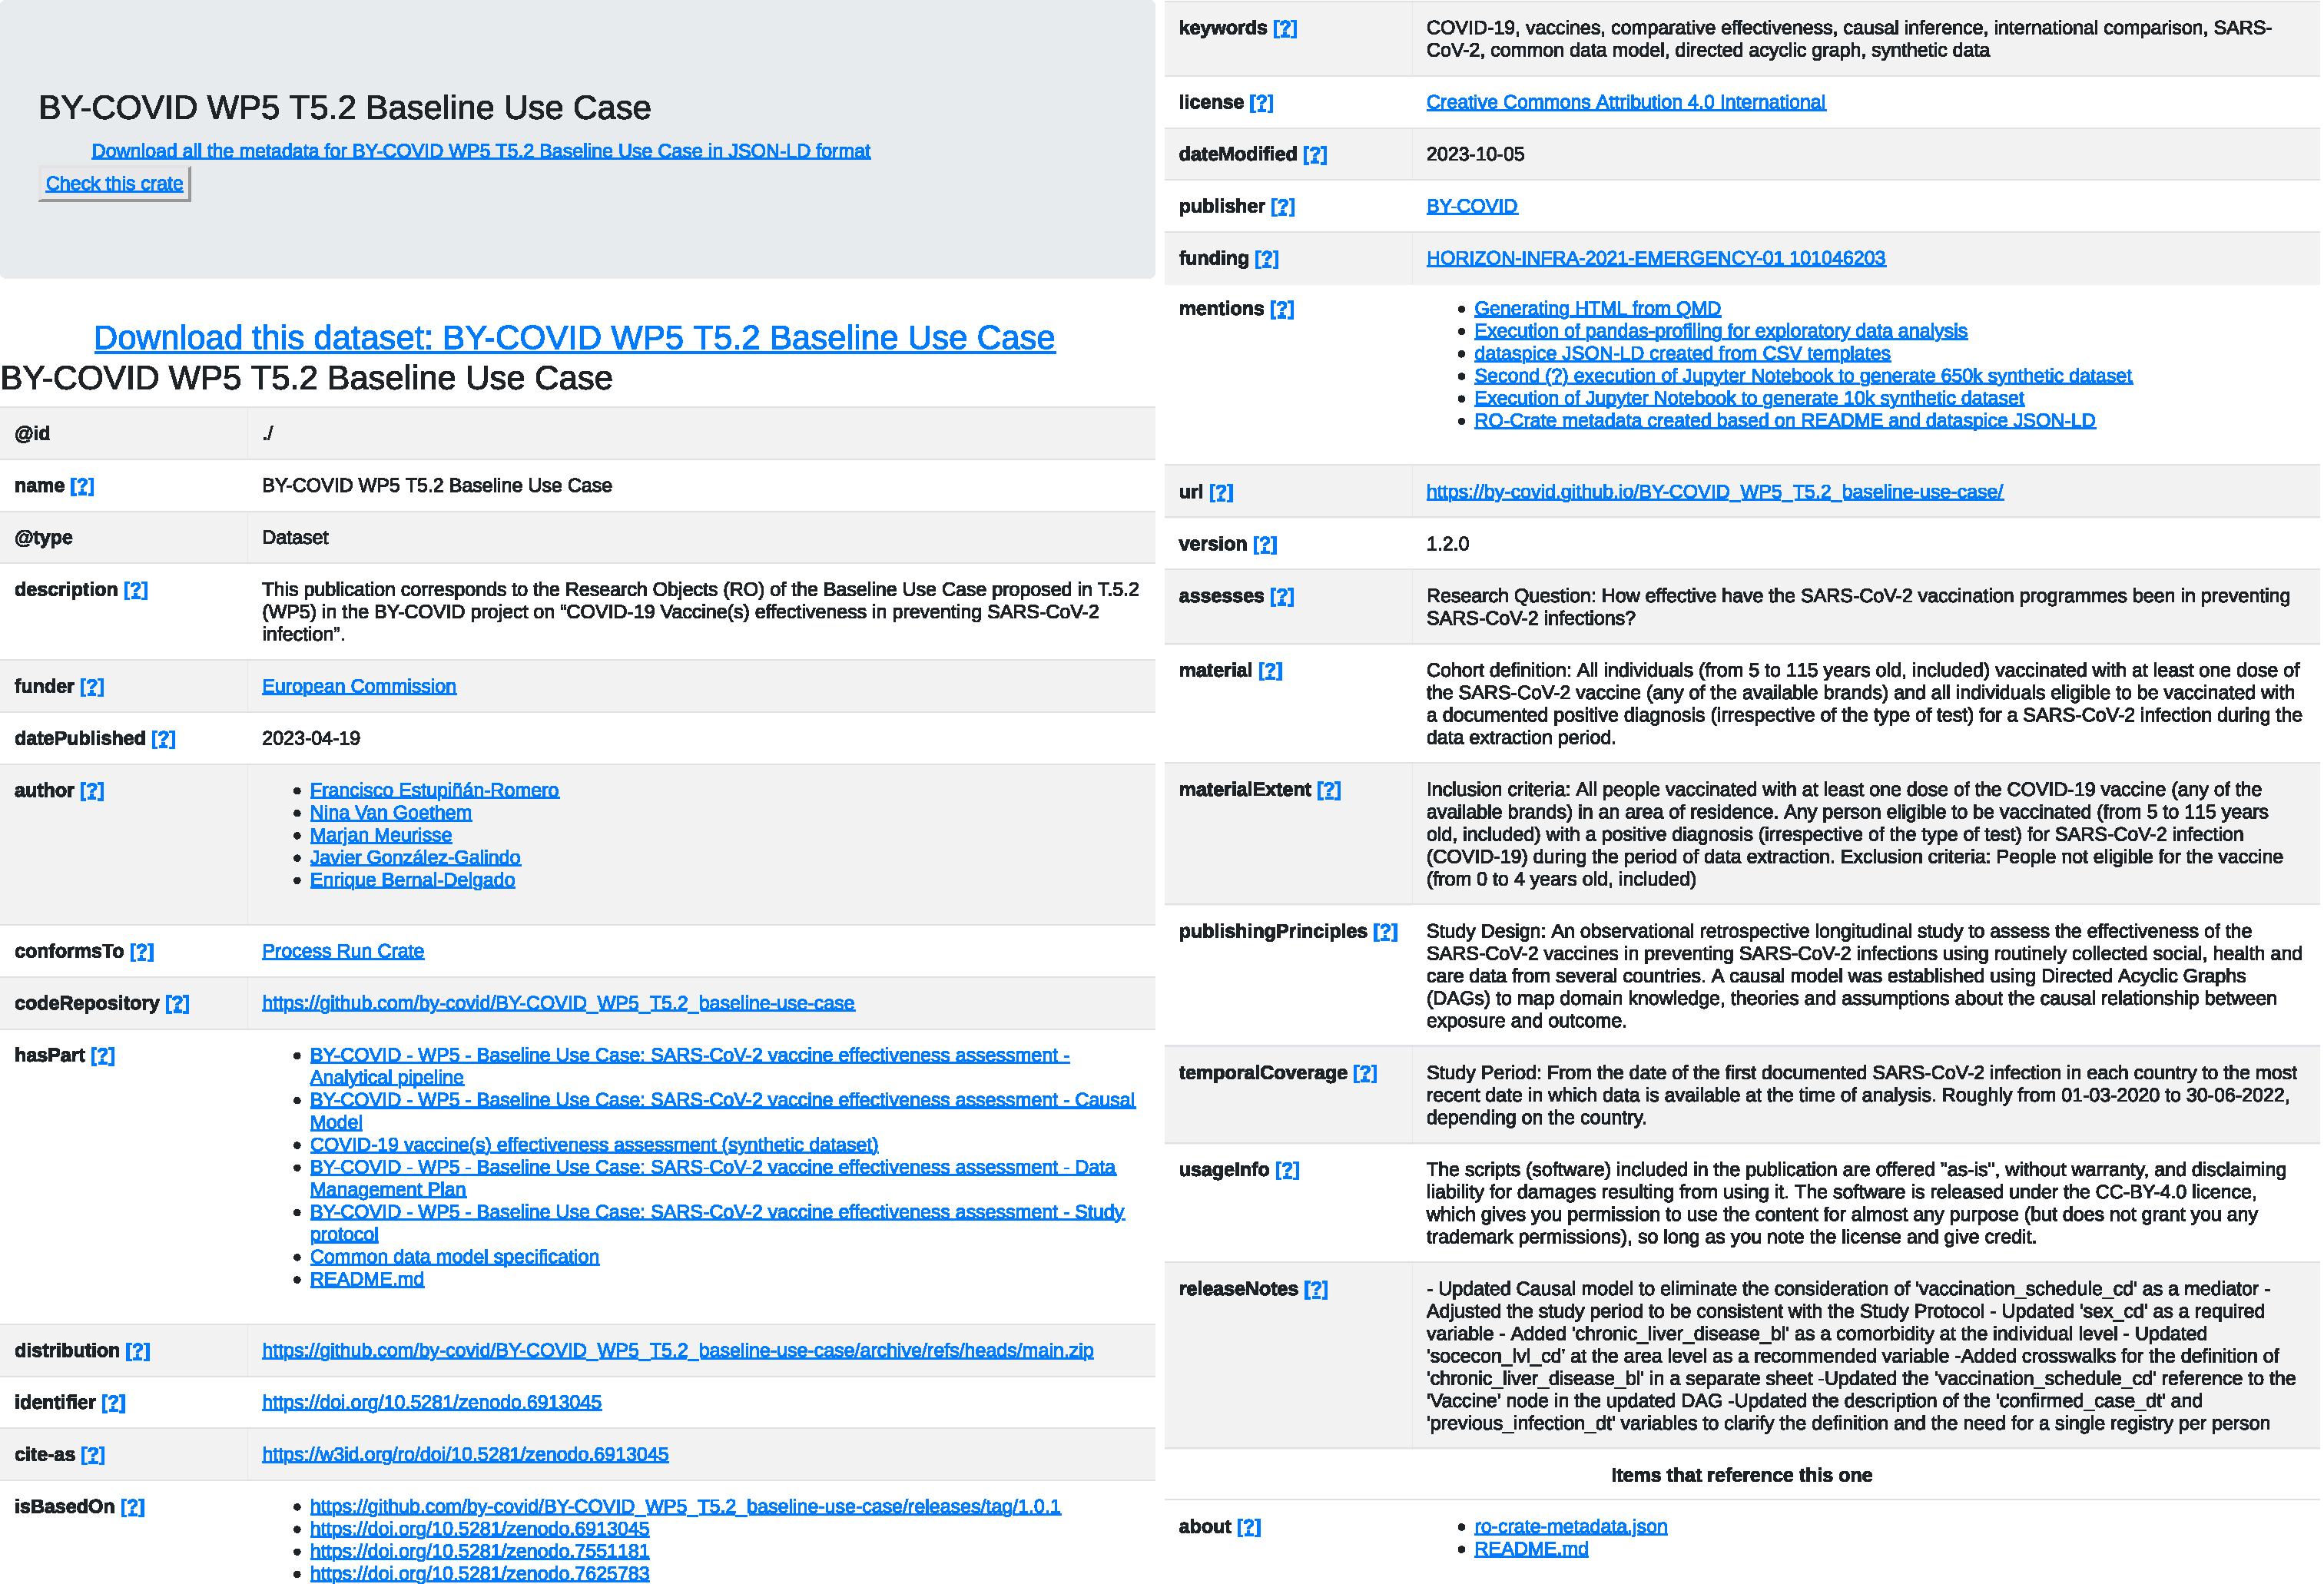
\includegraphics[height=\textheight]{figures/ch09/baseline-usecase.pdf}
  
    \caption[Example of RO-Crate using the Process Run Crate profile]{\footnotesize \textbf{Example of RO-Crate using the Process Run Crate profile} to
    describe a BY-COVID use case for modelling vaccine effectiveness \cite{Meurisse 2023}.
    The crate \emph{hasPart} multiple data entities, and \emph{mentions} several process runs according to the profile. The use case is further described with extra schema.org attributes like \emph{temporalCoverage}. Screenshot of RO-Crate preview HTML, modified for print from \url{https://w3id.org/ro/doi/10.5281/zenodo.6913045}
    }
  \label{ch61:fig:baseline-usecase}
\end{figure}
\end{landscape}

The community making WRROC involved multiple developers from different backgrounds and a variety of workflow systems. 
A lesson to learn from that experience is that even though RO-Crate profiles give additional rigidity (as discussed in section \vref{ch61:profiles}) that enable interoperability like the \emph{runcrate run} reproducibility in section \vref{ch54:runcrate}, profiles need to also ensure sufficient flexibility for individual implementations of different capabilities and purposes.
Profiles are therefore different from stricter type systems and bounded schemas as otherwise used by FDO implementations and Linked Data ontologies.

An interoperability challenge remains on how much flexibility to permit, as discussed in \vref{ch61:profiles}. However it is arguably more interoperable to have optional features defined by the community when needed, rather than individual vendor extensions -- giving common ground and graceful fallback. This practice is in line with FDO principle FDO-FDOR4 (\emph{can include other community defined and registered attributes}) \cite{Anders 2023} and FAIR principle RDA-R1.3-01M (\emph{Metadata complies with a community standard}) \cite{FAIR Maturity 2020}.


\subsubsection{Profiles should not need to define subclasses}

Part of RO-Crate's philosophy is to use Semantic Web technology while avoiding many of its pitfalls discussed in section \vref{ch3:semweb} and \vref{ch5:simplicity}. 
An unusual consequence of this is that extension profiles like WRROC end up reusing multiple types for the same entity.  For instance, the \emph{CreateAction} representing a \footurl{https://w3id.org/ro/wfrun/process/0.4}{process run} has an \emph{instrument} to either a \texttt{SoftwareApplication}, \texttt{SoftwareCourceCode} or \texttt{ComputationalWorkflow}. In the specialising profile for \footurl{https://w3id.org/ro/wfrun/workflow/0.4}{workflow run} the actual type of the instrument is however a combination: \texttt{["File", "SoftwareSourceCode", "ComputationalWorkflow"]}

Traditional ontology thinking such as with OWL and RDFS would be to create a class hierarchy, indeed both  \url{http://schema.org/SoftwareSourceCode} and \url{http://schema.org/MediaObject} (aliased as \texttt{File} in RO-Crate's JSON-LD) are subtypes of \url{http://schema.org/CreativeWork} which has most of the useful properties like \emph{author} and \emph{license}. It would however not be RO-Crate's job to modify the existing schema.org class hierarchy to inject artificial superclasses like \emph{ApplicationOrSourceCodeOrWorkflow}, neither would it be desirable to create a subproperty of \emph{instrument} with the intended \emph{domainIncludes}, as that means using custom terms that diverge from schema.org. 

It is an important part of the simplification of the Semantic Web in RO-Crate that consumers should not need to do any ontology retrieval or reasoning. For RO-Crate users it is therefore natural to occassionally combine types, enabling properties from both. schema.org is not a strict ontology with disjoint classes, so this usually do not cause any problem. It is however not desirable to re-iterate supertypes already defined within schema.org such as \emph{CreativeWork}. 

RO-Crate profiles like WRROC live are doing a combination of \emph{restrictions} (requiring the crate to have a particular entity) and \emph{extensions} (suggesting additional terms to use). By following the RO-Crate philosophy the profiles also reuse existing schema.org types as much as possible, adding a filtered overlay of their many properties, just like RO-Crate itself, and only adding terms where no appropiate alternative exist.

Listing \vref{ch61:wrroc-in-owl} shows an attempt to declare the partial WRROC requirements from the top of this section in OWL. In doing so it was necessary to introduce additional types for the profile and the action, in addition to anonymous union classes and inverse properties. It is clear that expressing a full RO-Crate profile in this matter would require a deep understanding of OWL ontologies and would require its own set of unit tests, and would not be inline with the RO-Crate philosophy of \emph{just enough Linked Data}.

\begin{listing}
  \footnotesize
  \begin{verbatim}
<https://w3id.org/ro/wfrun/process/0.4> 
  rdf:type owl:NamedIndividual, :ProcessRunCrateProfile ;
  rdfs:label "Process Run Crate profile 0.4"@en-gb .    
:ProcessRunCrateProfile rdf:type owl:Class ;
    rdfs:subClassOf :ROCrateProfile ,
      [ rdf:type owl:Restriction ;
        owl:onProperty [ owl:inverseOf dct:conformsTo ] ;    
        owl:allValuesFrom [ 
            rdf:type owl:Restriction ;
            owl:onProperty s:mentions ;
            owl:someValuesFrom :ProcessRunAction
          ]
      ] ;
    rdfs:label "Process Run Crate profile"@en-gb .
:ProcessRunAction rdf:type owl:Class ;
  owl:equivalentClass [ 
    rdf:type owl:Class;
    owl:intersectionOf ( 
      [ rdf:type owl:Class ;
        owl:unionOf ( s:ActivateAction s:CreateAction s:UpdateAction ) ]
      [ rdf:type owl:Restriction ;
        owl:onProperty s:instrument ;
        owl:someValuesFrom [ rdf:type owl:Class ;
            owl:unionOf ( s:SoftwareApplication s:SoftwareSourceCode
              bioschemas:ComptuationalWorkflow ) ]
      ] )
  ] ;
  rdfs:subClassOf s:Action ;
  rdfs:label "ProcessRunAction"@en-gb .
  \end{verbatim}
  \caption[Defining a Process Run action as an OWL equivalence class]{\textbf{Defining a Process Run action as an OWL equivalence class}. A versioned \texttt{:ProcessRunCrateProfile} is given a restriction in that the RO-Crate root which list the profile as \texttt{conformsTo} must \emph{mention} an action (one of \emph{ActivateAction},  \emph{CreateAction},  \emph{UpdateAction}) which \emph{instrument} have at least one instance of \emph{SoftwareApplication} \emph{SoftwareSourceCode} or \emph{ComptuationalWorkflow}. This OWL ontology uses equivalence classes as the WRROC types must be inferred and not declared in their JSON-LD \texttt{@id}.
  OWL Turtle snippet modified from \url{https://github.com/ResearchObject/workflow-run-crate/pull/69}
  
  }
 \label{ch61:wrroc-in-owl}
\end{listing}

However, that is not to say that such OWL rules cannot be generated from simpler definitions of RO-Crate profile requirements. Of future consideration is that the tool Crate-O's  \footurl{https://github.com/Language-Research-Technology/ro-crate-editor-profiles}{Editor profiles} (mainly for driving the UI form generations), and \footurl{https://linkml.io/linkml/}{LinkML} which can generate ShEx, SHACL, OWL and JSON-LD context from a concise YAML definition -- in coordination with validation as discussed in section \vref{ch61:fair-crates}.




\subsubsection{Linked data provenance models can be made approachable}

As dicussed in sections \vref{intro:rq3} and \vref{ch54:introduction}, the subject of capturing provenance from computational workflow executions is both diverse and mature, with most of the implementations coalescing on the W3C PROV data model \cite{Moreau 2013}, and in particular specializations of the OWL ontology serialization PROV-O \cite{Lebo 2013a}. Yet even with earlier approaches like Research Objects wfprov \cite{Belhajjame 2015}, D-PROV \cite{Missier 2013} and CWLProv \cite{Khan 2019}, the uptake of these technologies by scientific workflow systems is fragmented at best.

Given these approaches rely on Semantic Web technology and hierarchies of ontologies, it is not a far stretch to hypothesie that some of the challenges on uptake of Linked Data we discussed in section \vref{ch3:ld} and \vref{ch5:simplicity} also apply to the use of PROV-O by workflow systems developers. 

A core concern for workflow users is to get hold of and distribute their result data -- the exact computational structure is often of less concern as it is taken for given from the workflow definition. A change of focus from process-oriented to data-oriented will therefore also be beneficial for workflow provenance. 

Targeted workflow provenance models like Biocompute Objects (BCO) \cite{IEEE 2791-2020,Alterovitz 2018}, discussed in sections \vref{ch5:regulatorysciences} and \vref{ch54:bco-crate}, emphasise the \emph{context} of the workflow -- what is the purpose? What are possible inputs? What data sources are referenced?  BCO is being implemented by workflow management systems in Life Science domain including Nextflow and Galaxy, but is perhaps not deemed generic enough for other domains like earth sciences or astronomy.  While extensions are possible in BCO (e.g. \footurl{https://wiki.biocomputeobject.org/index.php?title=Extension-fhir}{FHIR}) they are separate from the rest of the descriptions and do not natively support Linked Data principles.

The aspect of documenting the context and human processing is also emphasised by Five Safes Crate \cite{Soiland-Reyes 2023f} as discussed in section \vref{ch54:trusted-workflow-run-crate}. Here the \cite{schema actions} are used to record the review process in a restricted environment for sensitive data, while also progressing the crate towards becoming a Workflow Run Crate. This model has built interest beyond workflow computations in the health data research area, amongst implementers who are not native speakers of FAIR principles or Linked Data technologies.

Section \vref{ch54:implementations} presented the range of workflow systems that have implemented WRROC, and section \vref{ch54:exemplary-use-cases} illustrated usage in the biomedical domain. While it is too early to tell to what extent WRROC is an approachable lightweight provenance model that can be implemented for many different research domains, the reception from those approaching it so far has been overwhelmingly positive. At the same time, new members of the WRROC community tend to contribute new requirements or adjustments that means the model is both maturing and evolving.


\subsubsection{Combining provenance and metadata models gives the best of both worlds}

The intention of Workflow Run Crate, and indeed RO-Crate overall, is not to replace all existing Linked Data descriptions of research data and workflows. Even if the format of RO-Crate is JSON-LD, and in theory can support any RDF vocabulary, that does not mean that doing so is the right design decision. The engineering principle of \emph{separation of concern} applies just as well to Linked Data formats which seem possible to integrate -- in other words, just because it is \emph{possible} to merge two knowledge graphs that does not mean they should be!

The FAIR community has a long history of developing metadata standards, ontologies and provenance models. Research domains have also developed specific vocabularies and formats for repository submissions (often CSV-based), and likewise domain-specific models for making their registered data available as FAIR resources (often RDF-based, now more frequently JSON). 

If we consider the lessons of evaluating FAIR Digital Objects and Linked Data in chapter \vref{chapter:fdo}, and the philosophy of RO-Crate from chapter \vref{chapter:ro-crate}, then it would seem important to facilitate proliferation of existing community standards, but also make their content more generally Findable and Accessible using a common overlay.

An approach that we have found useful with RO-Crate is therefore to propagate the existing provenance and metadata serializations, but also annotate their format and profiles in the RO-Crate metadata as not all formats are self-describing or well-known. General metadata (e.g. authors, license, subject) can then be extracted and replicated in the RO-Crate, increasing its coverage of the domain and making the metadata available to a wider set of technologies. 

One approach for this covered by section section \vref{ch54:process-run-crate-and-cpm-ro-crate-for-cancer-detection} describes how the PROV-based Common Provenance Model \cite{Wittner 2023a} is used together with RO-Crate, both as a container of identified PROV bundles and by replicating the overall computation structure in the WRROC profiles.  The full details are left in the PROV serialization that is carried along within the crate, and can be combined with distributed provenance of real-life processes such as transferring a biosample between a hospital and a lab. 

Likewise interoperability with existing models is important, and section \vref{ch54:prov} showed how WRROC provenance can be mapped back to PROV. Note that some of the workflow details could be lost or muddled in a generic mapping if they don't have a corresponding pattern in PROV -- for instance the expression of the workflow engine execution does not explicitly type it as such, that would require a particular PROV extension such as OPMW-PROV \cite{Garijo 2011}. 


\subsubsection{A strong community trumps semantically correctness}

The development of Workflow Run Crate was done as a community activity (section \vref{ch54:conclusion}), following the same pattern as RO-Crate itself (section \vref{ch5:community}) and many activities within the ELIXIR Europe life science network \cite{Harrow 2022}. 

When collectively building semantic models, particularly using ontology design patterns \cite{Hitzler 2016}, it can often take much longer to figure out what is the \emph{meaning} of a term (e.g.~its semantics) rather than how it should be formalised in an ontology language. In research domains this often comes down to considering redefining core concepts of the field itself, which in life sciences for instance easily turn into philosophical dialectic arguments \cite{Falk 2010}. 

The recently started Workflows Community Initiative has a working group for \footurl{https://workflows.community/groups/fair/}{FAIR computational workflows}, but before it is able to formalise the FAIR principles for workflows (building on \cite{Goble 2020}), the group had to discuss to length what is or is not a \emph{workflow}, and what makes it different from other research software.

While such fundamentals are important to get right, they should not become blockers for community progress. In the pragmatic take by the WRROC community for instance, a reverse argument was made that it is not so important if a workflow engine exist or not, but rather that we wanted to capture "workflowy" provenance. The principle of ``I know it when I see it'' does not just apply to censorship of obscene material \cite{Gewirtz 1996}, but also to semantic design. In designing WRROC and RO-Crate it was useful to be constrained by the \cite{schema.org} vocabulary, for instance the type \url{http://schema.org/HowTo} -- with current examples showing how to change tires on a car -- was also found adequate for describing a computational workflow and its steps in the Provenance Crate Profile (section \vref{ch54:provenance-run-crate}). 

This forced generalization may also have helped to make the model general enough for the different forms of workflow systems who implemented it, as each would have to ``squint'' slightly to map the WRROC concepts to their much more specific engine concepts. This also leads to fruitful community discussions and allowing reinterpretions of existing assumptions, placing the ``just enough Linked Data'' idea (section \vref{ch61:justenough}) into practice.
